\documentclass{scrreprt}
\usepackage[english]{babel}
\usepackage[T1]{fontenc}
\usepackage{lmodern}
\usepackage{blindtext}
\usepackage[utf8]{inputenc}
\usepackage{siunitx} %For unit handling%
\renewcommand{\familydefault}{\sfdefault}
\newcommand{\unit}[1]{\ensuremath{\, \mathrm{#1}}}
\usepackage{amssymb, amsmath, cancel, ulem, graphicx, float, tabularx, multirow, bm}
\usepackage{amsmath}

\setcounter{secnumdepth}{5}
\setcounter{tocdepth}{5}

\author{Urs Gerber\\09-921-156 \and Gian-Luca Mateo\\11-113-545}
\date{21th of March 2013}

\title{Airfoil in a wind channel}
\subtitle{Practical course report}

\begin{document}

\maketitle

\tableofcontents
\newpage

\chapter{Experiment: Airfoil in a wind channel}
\section{Introduction}
\subsection{Goal of the experiment}
The goal of this experiment is to determine the angle of attack where for a given airfoil the ratio of air drag to lift is optimal. Furthermore, the lift is to be calculated by measuring the pressure conditions on the surface of the airfoil.
\subsection{Theory}
\section{Experiment setup and execution}
\subsection{Used materials}
The materials used in this experiment are the following:
\begin{itemize}
\item A wind turbine
\item An airfoil with some holes from the surface to the sides (for measuring the pressure)
\item A balance which allows attaching a hinged airfoil
\item Some weights
\item A prandtl tube
\item A manometer
\end{itemize}

\subsection{Assembly}
For this experiment we have to measure three things. And for both of them, we need the wind speed, which is measured using the prandtl tube and left at that value for the whole experiment. Then, we need to measure the air drag of the airfoil at different angles of attack. We do this by arranging the assembly as shown in figure \ref{fig:assembly1}. Now, for every angle between $\ang{-20}$ and $\ang{+20}$ (in $\ang{5}$ steps) the drag is measured using the balance.
Next, we rearrange the assembly as shown in figure \ref{fig:assembly2} and measure the lift for the same angles as before. Last, without modifying the assembly, we proceed to measure the pressure conditions on the surface of the airfoil by attaching a manometer to the foil's holes.

\begin{figure}[H]
	\centering
  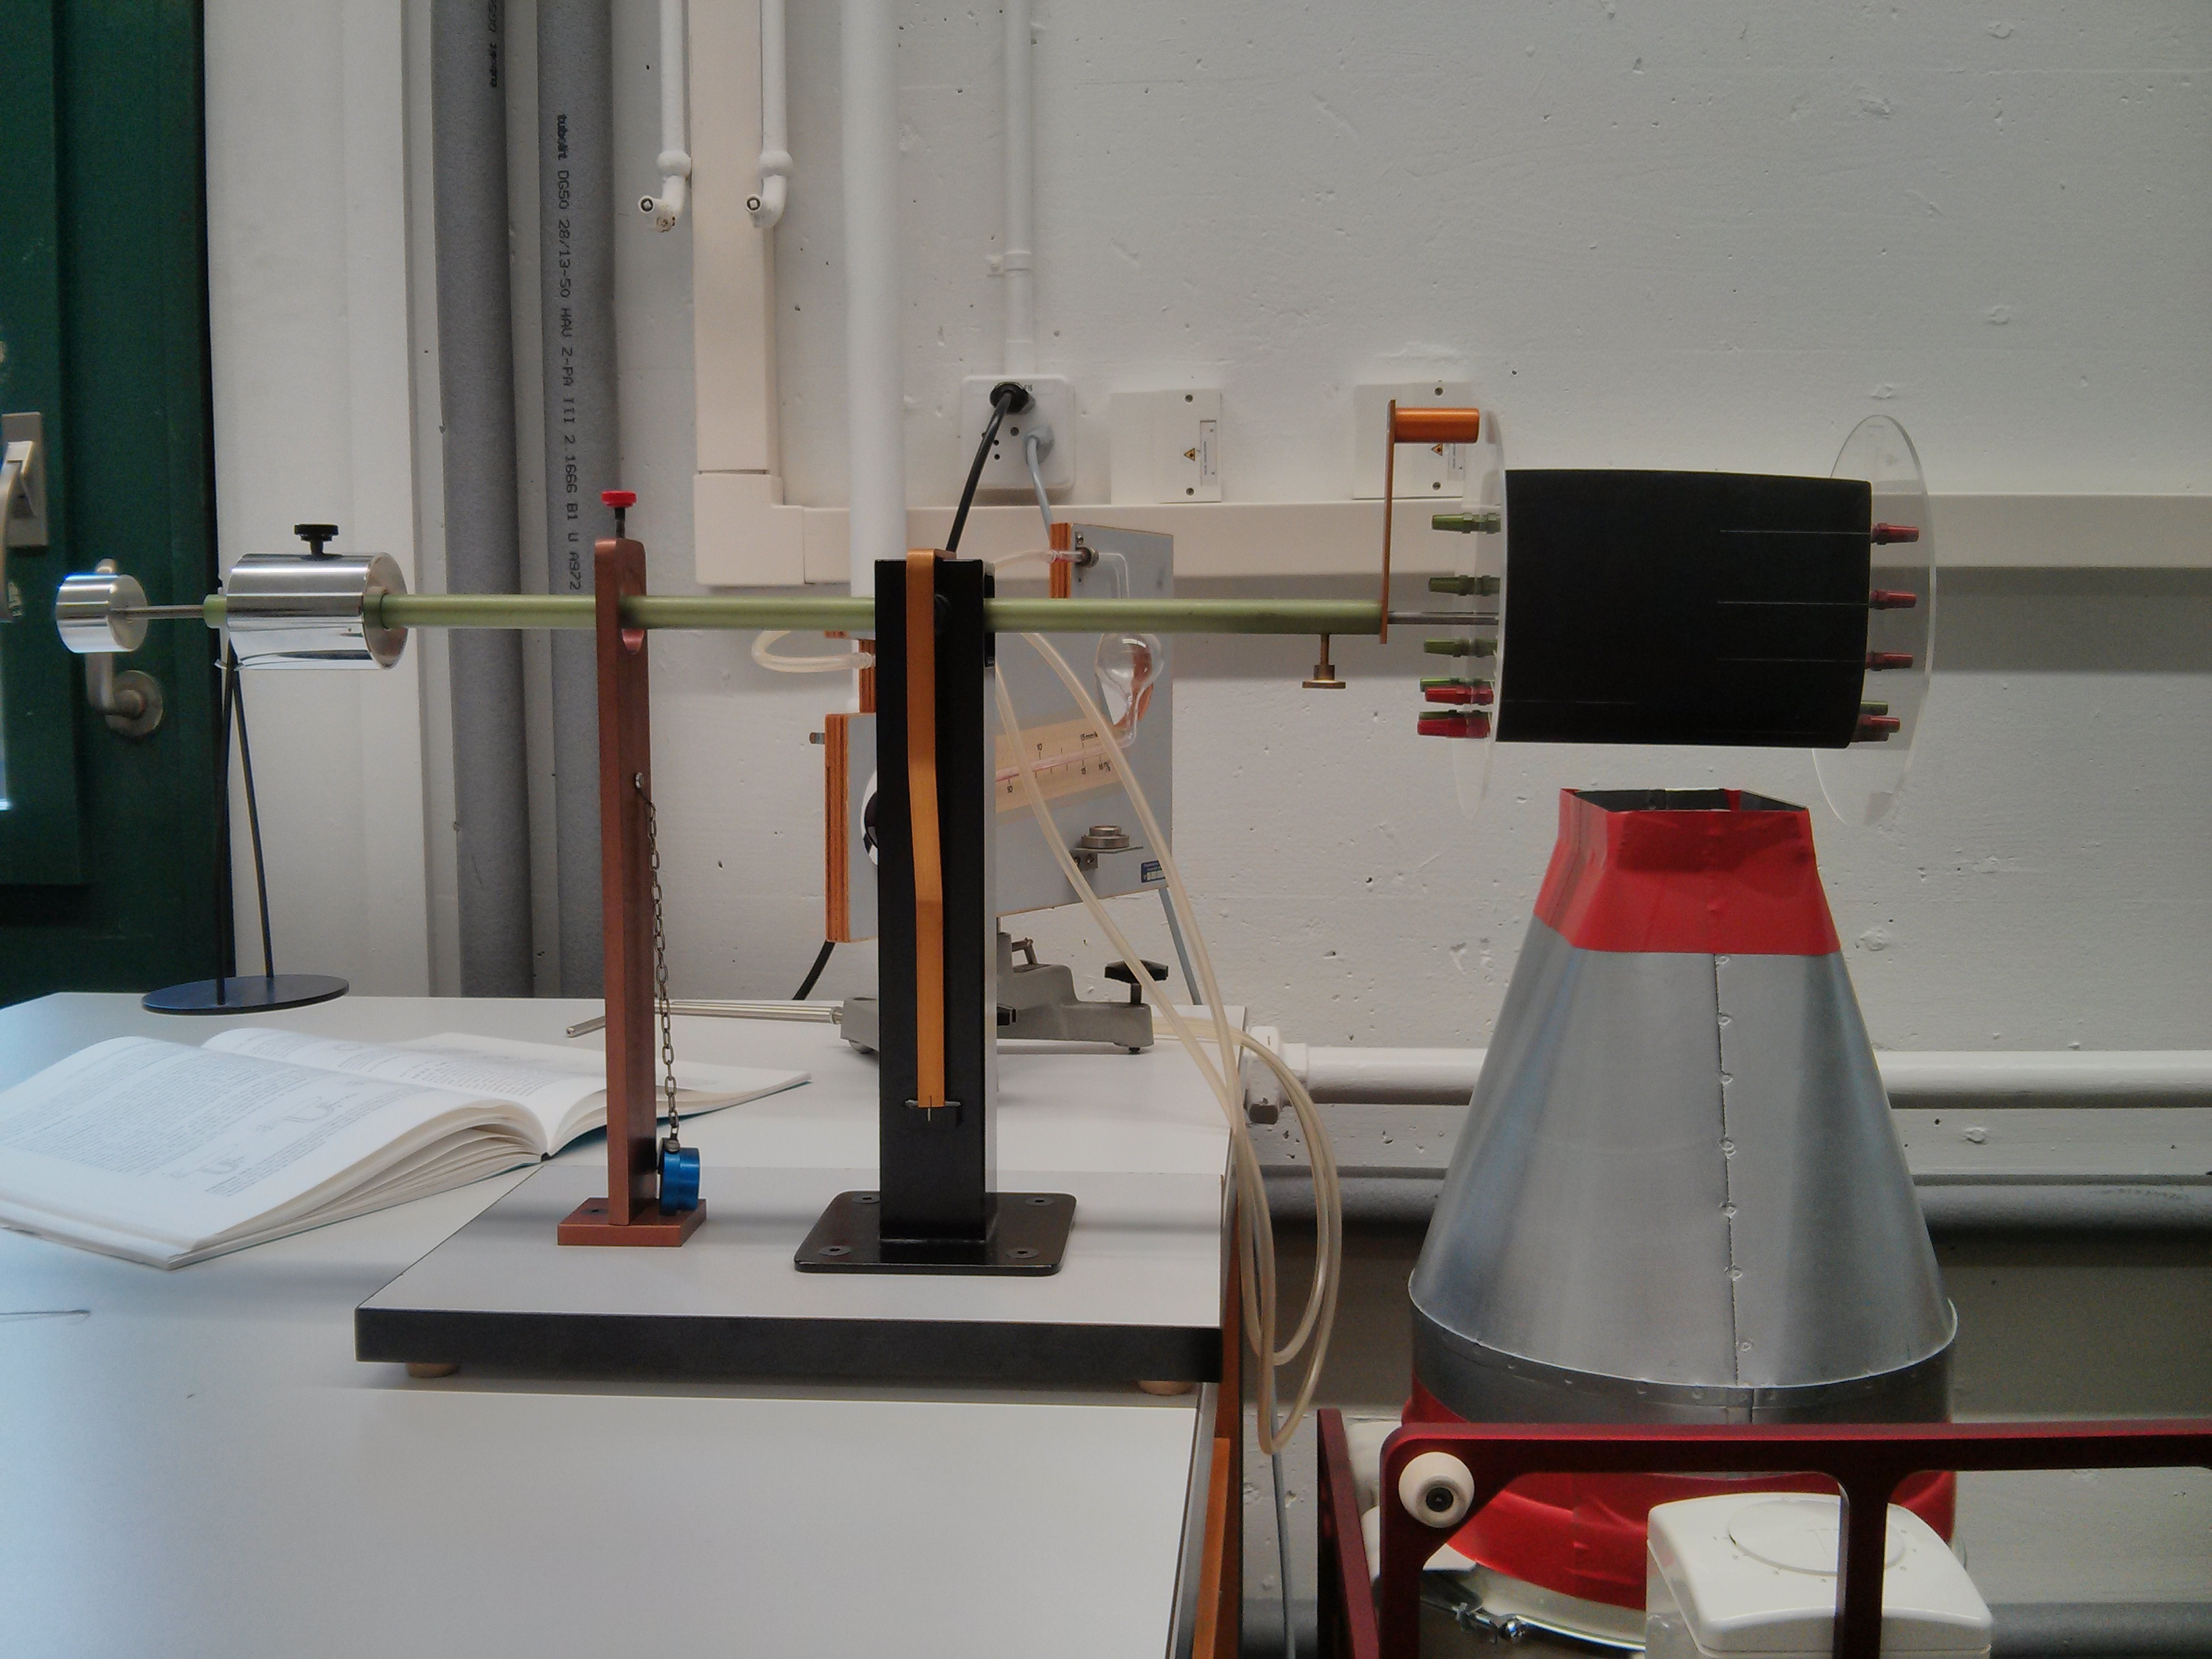
\includegraphics[width=0.9\textwidth]{img/assembly2.jpg}
	\caption{The Experiment Assembly}
	\label{fig:assembly2}
\end{figure}

\begin{figure}[H]
	\centering
  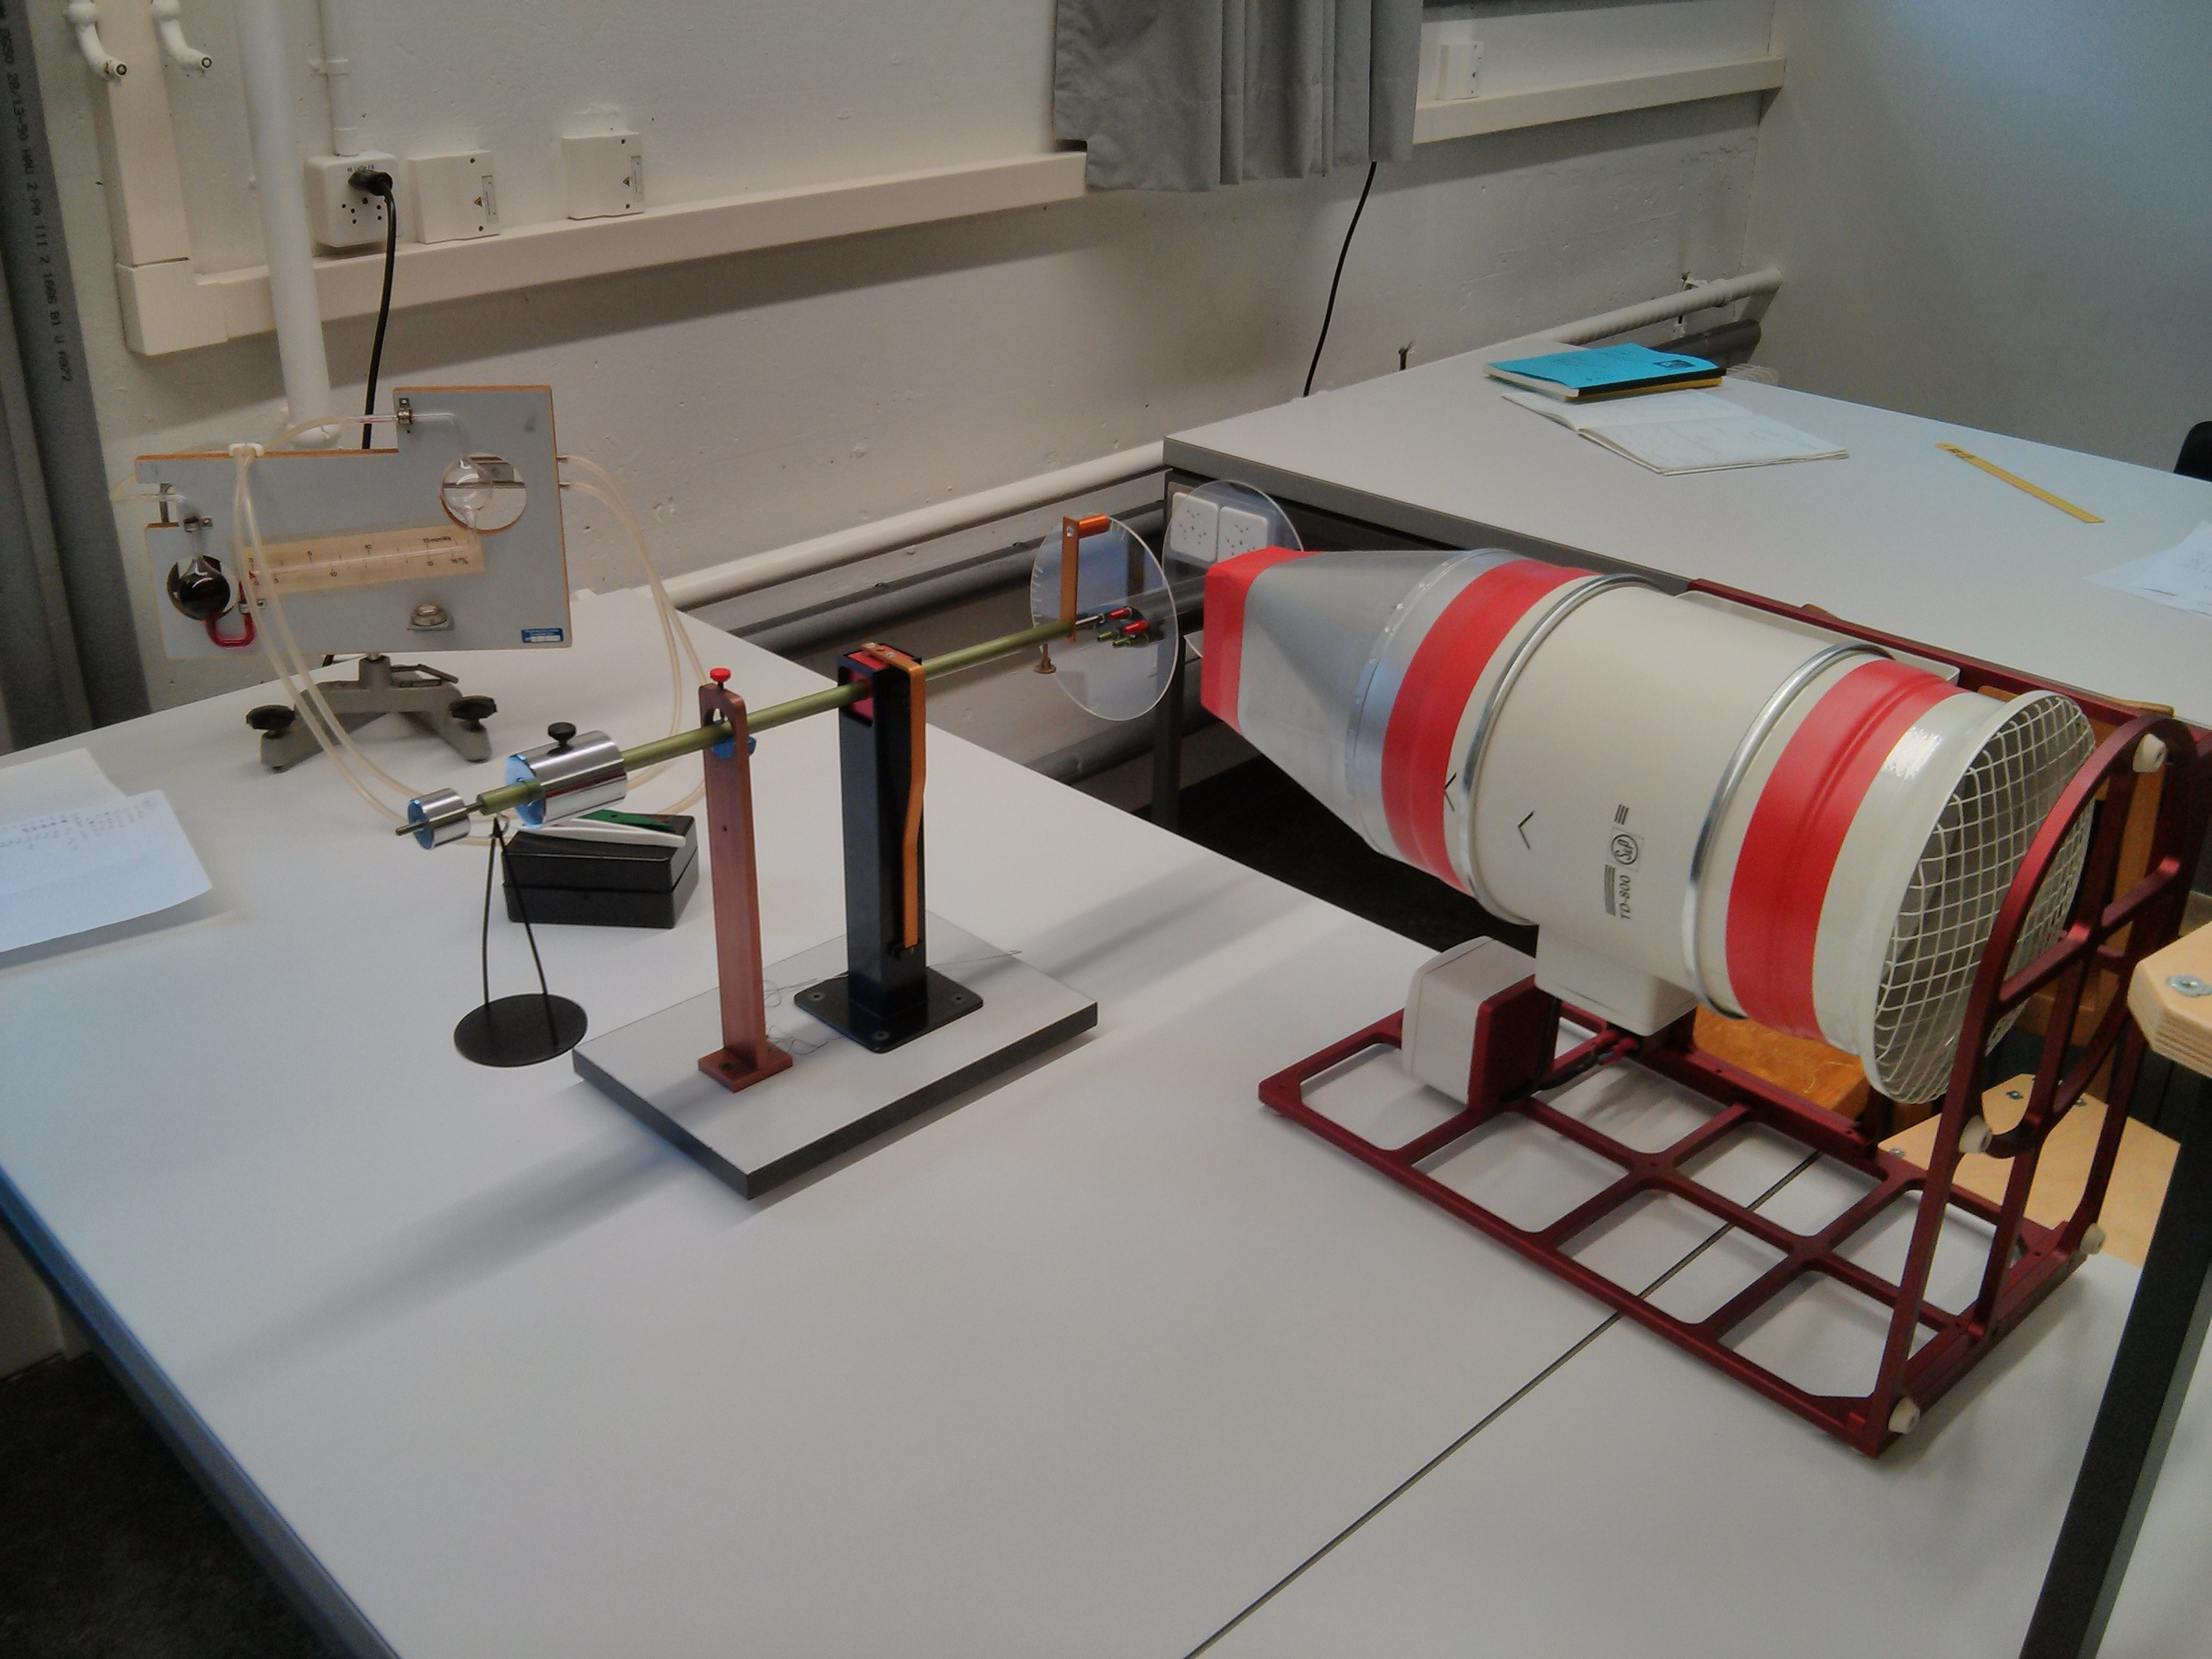
\includegraphics[width=0.9\textwidth]{img/assembly1.jpg}
	\caption{The Experiment Assembly}
	\label{fig:assembly1}
\end{figure}
\section{Measurements and analysis}
\section{Discussion}

\begin{thebibliography}{9}

\bibitem{physcript13}
  Peter Wurz,
  \emph{Anleitung zum Physikpraktikum}
  FS2013

\end{thebibliography}

\end{document}
